\claude{
\section{Monitoring and selection in learned systems}\label{sec:applied}
The applications test two uses of the same scalar statistic: monitoring independently measured changes and making decisions without access to full trajectories. CNN, VAE and grokking experiments address monitoring; policy, SSL and forecast selection address decisions. These tests establish empirical utility separately from absolute dimension recovery.

\subsection{Detecting restrictions on CNN parameter updates}\label{sec:cnn}
We train a 14,666-parameter convolutional neural network (CNN) on 10,000 CIFAR-10 images \citep{krizhevsky2009learning} for 10,000 SGD updates. At update 4,000, we reduce the learning rate, freeze layers, or prune weights. Reference runs continue unchanged or use a larger batch; separate transformed logs rescale or smooth the observation without altering training. MG receives only the norm of all parameters, which requires no extra network forward pass. Settings are $W=1{,}000$, stride 500, $E=20$, $\tau=1$, and $k=20$.

We choose detector settings on seeds 0--3 and test interventions of different strengths on new seeds 10--13. Independent measurements track update covariance participation ratio, the fraction of moving parameters and update magnitude. Freezing and pruning impose known restrictions on trainable or nonzero parameters. Learning-rate reduction changes the dynamics, but need not reduce invariant dimension; we assess its effect through the measured updates.

MG falls after strong restrictions on training. Freezing all but the classification head reduces it by a median 18.5\%, while update participation ratio falls by 43.5\%. Strong freezing and pruning produce median MG declines of approximately 12--19\%; reference-run medians range from near zero to increases of 13\%. Across intervention strengths, MG ratios and update participation-ratio changes have Spearman correlation 0.59. The two statistics need not agree: after 50\% pruning, MG falls while update participation ratio rises.

\begin{figure*}[t]
\centering
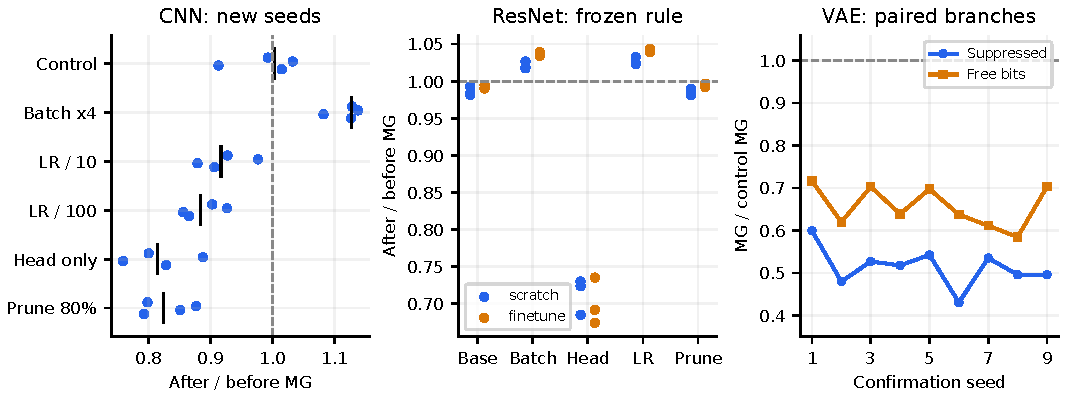
\includegraphics[width=.98\textwidth]{figures/applications.pdf}
\caption{\claude{MG under training interventions and latent-information suppression. Left: post/pre-intervention ratios on four CNN seeds; vertical marks indicate medians. Center: corresponding ResNet-18 ratios for scratch and pretrained initialization. Right: late VAE estimates relative to the shared low-regularization reference run, for suppression and free-bits branches on nine seeds. Points represent seeds; dashed lines indicate a ratio of one. Independent update and information measurements provide the references.}}
\label{fig:applications}
\end{figure*}

MG separates interventions from unchanged-training and increased-batch reference runs with AUC 0.93, versus 0.48--0.57 for trend crossings, lag-one correlation, and detrended standard deviation. IAAFT spectral surrogates yield 0.68. \appref{app:baselines} specifies the descriptive surrogate check, all scalar competitors, and alternative comparison sets.

\paragraph{Causal detection of training interventions.}
For window estimates $m_j$, we compare the median over the latest $M$ windows with the median over the preceding $B$ windows:
\begin{equation}
D_j=\frac{\median(m_{j-M+1},\ldots,m_j)}
{\median(m_{j-M-B+1},\ldots,m_{j-M})}-1.
\label{eq:detector}
\end{equation}
We choose $M=2$, $B=3$, and a detection threshold of $D_j<-0.0883$, a drop of 8.83\%. Only completed windows enter the rule. The first threshold crossing defines a detected change. It is correct if it occurs within 5,000 updates after the intervention; an earlier crossing is a false positive. Competing statistics use the same selection procedure.

MG detects 27/28 strong interventions with 0/16 reference false positives, while normalized increments give 28/28 and 0/16 (Table~\ref{tab:detectors}). MG detects 8/28, 16/28, and 22/28 within 500, 1,000, and 2,000 updates. On ten additional seeds with shifted intervention times, it gives 19/30 detections and false positives in five of ten reference runs, versus 30/30 and zero for absolute increments. The weaker result on shifted intervention times limits transfer of the original threshold. Runs sharing a seed are paired observations; \appref{app:baselines} gives the comparison details.

\begin{table}[t]
\centering\small
\caption{\claude{All scalar features with the same fixed block detector. Hits use a 5,000-update horizon. False positives are reference records with any threshold crossing; delay is the median over detected events. Four held-out seeds are shared across interventions and reference runs.}}
\label{tab:detectors}
\begin{tabular}{lrrr}
\toprule
Feature & Detected & FP & Delay \\
\midrule
MG & 27/28 & 0/16 & 1,000 \\
Abs. increments & 27/28 & 0/16 & 500 \\
Norm. increments & 28/28 & 0/16 & 1,500 \\
Perm. entropy & 28/28 & 7/16 & 1,500 \\
Sample entropy & 28/28 & 4/16 & 1,500 \\
Spectral entropy & 4/28 & 2/16 & 2,750 \\
Trend crossings & 15/28 & 5/16 & 1,000 \\
Lag-one corr. & 0/28 & 0/16 & --- \\
Detrended std. & 28/28 & 10/16 & 500 \\
Level & 4/28 & 0/16 & 1,000 \\
\bottomrule
\end{tabular}

\end{table}

\subsection{Transferring the detector to ResNet-18}
We transfer the parameter-norm observable, MG settings, and detection threshold to ResNet-18 \citep{he2016deep}, without retuning. Training uses the full CIFAR-10 training set, either from scratch or from ImageNet-pretrained weights, with three new seeds in each setting. Freezing the backbone while continuing to train the head reduces MG by a median 27.6\% and 30.8\%, respectively. The detector identifies all six freezing events with no false positives in 24 reference records.

The freezing result transfers from about 15 thousand to 11 million parameters. The same rule misses learning-rate reductions and pruning; layer norms and random projections also introduce false positives. Transfer therefore depends on the event and observable.

\subsection{Tracking latent information in a text VAE}\label{sec:vae}
A text variational autoencoder (VAE) learns to reconstruct Penn Treebank sentences \citep{marcus1993building} through a 16-dimensional Gaussian latent code. Its encoder and decoder use gated recurrent units \citep{bowman2016generating}; the model has 276,016 parameters and trains on 6,000 sentences. We test whether MG detects reduced dependence of decoder outputs on the latent code.

After 1,024 shared updates with Kullback--Leibler (KL) regularization weight $\beta=0.01$, we split training into three branches: keep that weight, raise it to one, or use $\beta=1$ with a free-bits objective. The free-bits objective excludes low-KL latent coordinates from further KL penalization. All branches train until update 3,072.

MG uses the reconstruction negative log-likelihood (NLL) per token on 16 fixed evaluation sentences, with fixed latent sampling noise. It has no access to KL or the independent references. On a larger set of 256 fixed evaluation sentences, the references estimate latent mutual information and the change in decoder outputs after shuffling codes between sentences. A joint decline means that less information is retained and used through the latent code.

The information-loss criterion is met on all nine test seeds. MG declines more strongly in the high-regularization branch than in the matched reference on every seed: their median late MG ratio is 0.517, with a 95\% seed-bootstrap interval [0.480, 0.542]. Free bits partially preserves both information and decoder dependence. MG is then higher than in the suppressed branch on all nine seeds, with median ratio 1.286 [1.179, 1.418]. The two branches use the same KL weight but retain different amounts of information. MG distinguishes them from reconstruction logs alone.

Standard deviation and spectral entropy also detect information loss on all nine seeds. Using MG to schedule reference checks is less successful: a separate cyclic-VAE test finds 28/41 transitions, versus 38/41 for periodic checks. Tracking information loss and scheduling measurements are distinct tasks. 

\subsection{Detecting changes during grokking}
Parameter-norm MG falls near generalization in four modular-arithmetic runs when its windows match the resolution of stored trajectory sketches. Those sketches independently show a reversible fall in detrended covariance participation ratio. Across analysis settings, 24/26 usable comparisons separate these runs from two references, but reuse the same trajectories. Roughness changes are stronger. A memorizing run also simplifies, while the full-batch setting does not reproduce the effect. MG detects a transition here; its decrease is not specific to generalization.

\subsection{Selecting Walker2d policies under actuator shifts}
PPO policies in Walker2d \citep{schulman2017proximal,todorov2012mujoco} show lower action-log MG under moderate action smoothing in two five-seed series. This does not imply simpler whole-body motion. We additionally select among 16 saved policies per seed using three nominal rollouts and a shared reward/survival gate. On four held-out fine-tuning seeds, minimum action-norm MG gives deployment return 4.313 versus 4.005 for nominal-reward selection under hidden actuator lag/noise; completion rises from 80.0\% to 90.8\%. Spectral entropy performs better (4.480, 97.5\%), and a pilot-selected fixed configuration nearly matches MG (4.310). This is exploratory policy selection, not demonstrated curriculum or training acceleration; \appref{app:rl_selection} reports all comparisons and shared-initial-policy limitations.

\subsection{Selecting SSL configurations from gradient logs}\label{sec:ssl}
Joint-embedding self-supervised learning (SSL) trains representations to agree across augmented views. Agreement alone can admit collapsed solutions that map different images to the same representation \citep{chen2021simsiam}; training loss is therefore an unreliable guide to representation quality \citep{garrido2023rankme}. We test whether gradient-norm MG can guide configuration choice without extracting embeddings from each evaluated model. The MNIST experiment compares 29 configurations across four objectives using a 784--256--256 MLP encoder. We choose the log and score direction from labeled development runs, then freeze the rule for five test seeds. Applying it requires no labels.

MG selects configurations with low average regret and ranks them more accurately than encoder RankMe, the tested $\alpha$-ReQ slope and LiDAR implementations \citep{garrido2023rankme,agrawal2022alphareq,thilak2024lidar}. Table~\ref{tab:ssl_campaign} reports correlations and selection regret. Embedding spread has the highest mean correlation; several simple scalar features remain competitive. The benefit is useful selection from a saved gradient log without an embedding pass. \appref{app:campaign} details the single-dataset scope, proxy implementations and uncertainty.

\subsection{Warning of loss spikes in transformer training}
In a two-layer transformer trained on modular addition, MG of log-loss warns of most test spikes within the specified horizon. It has higher AUROC than the tested attention-logit and attention-entropy monitors. Roughness detects more events at the same false-positive rate for less computation (Table~\ref{tab:spikes_campaign}). This result supports detecting the slingshot regime from scalar logs. Preventing spikes and transferring the rule to language models remain untested (\appref{app:campaign}).

\claude{
\subsection{Forecast model selection from single-neuron recordings}\label{sec:forecast_utility}
Can a scalar record identify a suitable forecasting model without fitting every candidate to held-out data? We train a selector that uses MG from 2,048 observations of one neuron to choose among eight forecasters. The selected model predicts the next 32 observations. Candidates include persistence, mean and cycle forecasts, linear regression, nearest-neighbor prediction and a nonlinear feature model. We fit the selector on 18 initialization seeds and freeze it for evaluation. Networks that miss their training targets remain included; the task is to predict the activity they actually produce (\appref{app:forecast_utility}).

MG has lower mean NMSE than TwoNN and Levina--Bickel selection; the difference from held-out search is unresolved (Table~\ref{tab:forecast_all}). A query subsample preserves every full-MG choice on further runs at lower cost (Table~\ref{tab:forecast_utility}). Selectors using held-out forecast errors can be more accurate. The saving concerns selection from an available record.
\begin{table}[t]
\centering\small
\caption{\claude{Forecast selection on 20 new seeds, eight tasks per seed. NMSE uses prefix variance. Time includes selection and the chosen fit on 12 matched inputs; a dash means not benchmarked. Acquisition and offline selector training are excluded.}}
\label{tab:forecast_utility}
\begin{tabular}{lrr}
\toprule
Selector & NMSE & Time (ms) \\
\midrule
MG & 0.0364 & 199.1 \\
MG, $q=128$ & 0.0364 & 12.2 \\
Held-out model search & 0.0407 & 45.3 \\
Cheap + held-out search & 0.0338 & --- \\
Held-out errors + MG & 0.0317 & --- \\
\bottomrule
\end{tabular}

\end{table}
}

}
